% Created 2023-03-04 Sat 15:13
% Intended LaTeX compiler: lualatex
\documentclass[11pt]{article}
\usepackage[margin=0.5in]{geometry}
\usepackage{syntax}
\usepackage{pdfpages}
\usepackage{tcolorbox}
\usepackage{etoolbox}
\usepackage{environ}
\usepackage[ruled]{algorithm2e}
\let\oldtabular\tabular
\let\oldendtabular\endtabular
\NewEnviron{tabular2}[1]{\tcbox[left=0mm, right=0mm, top=0mm, bottom=0mm]{\oldtabular{#1}\BODY\oldendtabular}}
\BeforeBeginEnvironment{minted}{\begin{tcolorbox}}%
\AfterEndEnvironment{minted}{\end{tcolorbox}}
\BeforeBeginEnvironment{verbatim}{\begin{tcolorbox}}%
\AfterEndEnvironment{verbatim}{\end{tcolorbox}}
\usepackage{graphicx}
\usepackage{longtable}
\usepackage{wrapfig}
\usepackage{rotating}
\usepackage[normalem]{ulem}
\usepackage{amsmath}
\usepackage{amssymb}
\usepackage{capt-of}
\usepackage{hyperref}
\usepackage{minted}
\usepackage{physics}
\author{David Lewis}
\date{\today}
\title{lec17}
\hypersetup{
 pdfauthor={David Lewis},
 pdftitle={lec17},
 pdfkeywords={},
 pdfsubject={},
 pdfcreator={Emacs 28.2 (Org mode 9.6)}, 
 pdflang={English}}
\begin{document}

\maketitle

\section*{1.}
\label{sec:org7c2f43e}
\begin{table}[htbp]
\label{data}
\centering
\begin{tabular2}{rrr}
ID & y & haty\\
\hline
1 & 1 & -1\\
2 & -1 & 1\\
3 & -1 & 1\\
4 & 1 & -1\\
5 & -1 & 1\\
6 & 1 & 1\\
7 & -1 & -1\\
8 & 1 & 1\\
\end{tabular2}
\end{table}

\subsection*{a.}
\label{sec:org63a388c}
I went ahead and computed the values anyway with python:
\begin{minted}[fontsize=\scriptsize]{python}
right = 0
for i in data:
    if i[1] == i[2]:
        right += 1
accuracy = right/len(data)
error_rate = 1 - accuracy
out = [["accuracy:", accuracy],["error rate:", error_rate]]
return out
\end{minted}

\begin{center}
\begin{tabular2}{lr}
accuracy: & 0.375\\
error rate: & 0.625\\
\end{tabular2}
\end{center}
\subsection*{b}
\label{sec:org75b06a1}
\begin{center}
\begin{tabular2}{r|r|r}
 & True & \\
\hline
predicted & 1 & -1\\
\hline
1 & 2 & 3\\
-1 & 2 & 1\\
\end{tabular2}
\end{center}
\begin{itemize}
\item True positive: 2
\item False positive: 3
\item True negative: 1
\item false negative: 2
\end{itemize}

\subsection*{c, d}
\label{sec:org61e2793}
\begin{itemize}
\item Sensitivity = true positive rate = 2/5
\item Specificity = true negative rate = 1/3
\end{itemize}

The classifier does not have very good performance. It is more likely to return
a false positive or false negative than a true positive or negative.
\subsection*{e.}
\label{sec:orga9a0938}
\begin{itemize}
\item Accuracy = precision = (2/(2+2)) = 2/4
\item recall = 2/(2+3) = 2/5
\end{itemize}
The accuracy and recall are very far from 1, this is a bad classifier.
\subsection*{f.}
\label{sec:orgff414be}
\(F1 = \frac{2 \cdot pred \cdot recall}{pred + recall} = \frac{8/20}{18/20} = 1/2\)
\section*{2.}
\label{sec:org4716197}
\subsection*{a-b}
\label{sec:orgd8b2b38}
\begin{table}[htbp]
\caption{\label{t1}table 2}
\centering
\begin{tabular2}{rrrrr}
ID & y & p & p >= 0.8 & p >= 0.5\\
\hline
1 & -1 & 0.9 & -1 & -1\\
2 & 1 & 0.8 & 1 & -1\\
3 & -1 & 0.5 & 1 & 1\\
4 & 1 & 0.3 & 1 & 1\\
\end{tabular2}
\end{table}

\begin{table}[htbp]
\caption{\label{t2}table 2}
\centering
\begin{tabular2}{rrrrr}
ID & y & p & p >= 0.8 & p >= 0.5\\
\hline
1 & -1 & 0.5 & 1 & 1\\
2 & 1 & 0.8 & 1 & -1\\
3 & -1 & 0.9 & -1 & -1\\
4 & 1 & 0.7 & 1 & -1\\
\end{tabular2}
\end{table}

\begin{minted}[fontsize=\scriptsize]{python}
def true_false(name, data):
    true_positives_8 = 0
    false_positives_8 = 0
    true_positives_5 = 0
    false_positives_5 = 0
    for i in data:
            if i[3] == 1:

                if i[1] ==1:
                    true_positives_8 += 1
                else:
                    false_positives_8 += 1
            if i[4] == 1:
                if i[1] == 1:
                    true_positives_5 += 1
                else:
                    false_positives_5 += 1

    def recall(r1 ,r2):
        return r1/(r1+r2)

    out = [[name, "p >= 0.8", "p >= 0.5"],
        ["true positive rate", recall(true_positives_8, false_positives_8), recall(true_positives_5, false_positives_5)],
        ["false positive rate", recall(false_positives_8, true_positives_8), recall(false_positives_5, true_positives_5)]
        ]
    return out
return true_false("Table 1", table1) + true_false("Table2", table2)
\end{minted}

\begin{center}
\begin{tabular2}{lrr}
Table 1 & p >= 0.8 & p >= 0.5\\
true positive rate & 0.6666666666666666 & 0.5\\
false positive rate & 0.3333333333333333 & 0.5\\
Table2 & p >= 0.8 & p >= 0.5\\
true positive rate & 0.6666666666666666 & 0.0\\
false positive rate & 0.3333333333333333 & 1.0\\
\end{tabular2}
\end{center}

\subsection*{c-d}
\label{sec:org263a8ee}
\begin{minted}[fontsize=\scriptsize]{python}
import matplotlib.pyplot as plt
p1 = data[1][1], data[2][1]
p2 = data[1][2], data[2][2]
p3 = data[4][1], data[5][1]
p4 = data[4][2], data[5][2]
fig,(axes1, axes2) = plt.subplots(1, 2, sharex=True, sharey=True)
axes1.plot((p1[0], p3[0]),[p1[1], p3[1]])
axes1.scatter((p1[0], p3[0]),[p1[1], p3[1]])
axes1.set_title("P >= 0.8")
axes2.plot((p2[0], p4[0]),[p2[1], p4[1]])
axes2.scatter((p2[0], p4[0]),[p2[1], p4[1]])
axes2.set_title("P >= 0.5")
fig.supxlabel("True Positive rate")
fig.supylabel("False Positive rate")

plt.show()
\end{minted}
\begin{center}
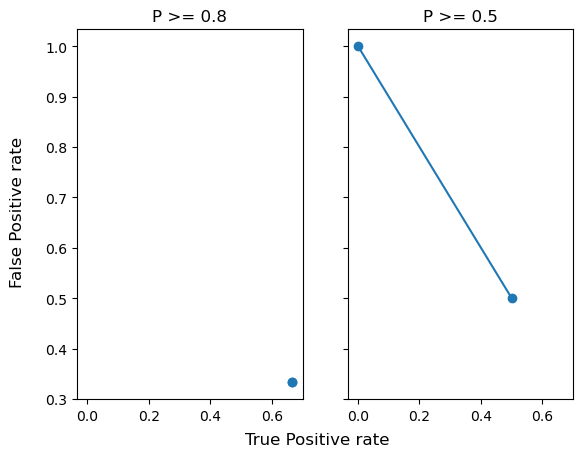
\includegraphics[width=0.8\textwidth]{./.ob-jupyter/56aa79352d69672f8941ac1a635528d4d749ff50.png}
\end{center}

The P >= 0.8 classifier is \textasciitilde{}66\% likely to have a true positive, which did not
change across training data.  The P >= 0.5 classifier actually had a negative
ROC curve, which is probably impossible, but implies that as the false positive
rate goes down, the true positive rate actually increases. There isn't enough
data to make a good prediction either way, but it does appear that the P >= 0.8
classifier is more effective.


\subsection*{3.}
\label{sec:org1e38c58}
5 fold validation implies 5 separate ``folds'' or groups of test data as follows:

\begin{center}
\begin{tabular2}{rll}
fold & train & test\\
\hline
1 & \{id\textsubscript{3}, \ldots{} id\textsubscript{10}\} & \{id\textsubscript{1}, id\textsubscript{2}\}\\
2 & \{id\textsubscript{1}, i\textsubscript{2}, id\textsubscript{5}, \ldots{} id\textsubscript{10}\} & \{id\textsubscript{3}, id\textsubscript{4}\}\\
3 & \{id\textsubscript{1}, \ldots{} id\textsubscript{4}, id\textsubscript{7}, \ldots{} id\textsubscript{10}\} & \{id\textsubscript{5}, id\textsubscript{6}\}\\
4 & \{id\textsubscript{1}, \ldots{} id\textsubscript{6}, id\textsubscript{9}, id\textsubscript{10}\} & \{id\textsubscript{7}, id\textsubscript{8}\}\\
5 & \{id\textsubscript{1}, \ldots{} id\textsubscript{8}\} & \{id\textsubscript{9}, id\textsubscript{10}\}\\
\end{tabular2}
\end{center}
\subsection*{4.}
\label{sec:org7713a35}
\begin{itemize}
\item Boostrapping selects sets of data of a fixed size an arbitrary number of
times, this forms a new ``fake'' training set for each member of the ensemble (a
set of weak learners)
\item In boosting, data in random is assigned a weight based on the performance of
the previous classifier, (initialized equal). This method iterates upon
previous classifiers by increasing the weight of data that is misclassified. This technique aims to minimize
bias, while bagging aims to reduce variance.
\item Bagging reduces the variance by averaging output of many classifiers that are
trained on random samples of the data. Using the independent and
representative nature of random samples, prevents weak learners from being
fully independent.
\item Boosting reduces the bias by assigning weights to data that is incorrectly
classified. This successive optimization minimizes the amount of prejudiced
results (bias).
\end{itemize}
\end{document}
